\documentclass[12pt]{article}
% Some custom commands to make typing easier. Feel free to add to it


% quick homomorphism
\newcommand{\homo}[1]{\varphi (#1)}
% quick inverse
\newcommand{\inv}[1]{#1^{-1}}
% quick generating set
\newcommand{\genset}[1]{\langle #1 \rangle}
% split problem into multiple parts
\newcommand{\spl}{\rule{\textwidth}{0.4pt}}
% quick normal subgroup
\newcommand{\nsub}{\trianglelefteq}
% quick Z/nZ
\newcommand{\znz}[1]{\mathbb{Z\text{/#1}Z}}
% quick stirling numbers
% \newcommand{\squig}{\genfrac{\lbrace}{\rbrace}{0pt}{}}
\newcommand{\squig}[2]{\left\{{#1 \atop #2}\right\}}


% quick projective surface
\newcommand{\proj}[1]{\mathbb P^{#1}(\mathbb C)}
% quick elliptic curve
\newcommand{\ellip}{E(\mathbb{C})}
% quick ramification
\newcommand{\ram}[1]{e_{#1}}

% todo list
\usepackage[color=yellow]{todonotes}
\newcommand{\tbd}[1]{\todo[inline]{#1}
\addcontentsline{toc}{subsubsection}{TODO}}

% scaling tikz
\usepackage{adjustbox}

% format bullets
% \usepackage[shortlabels]{enumitem}

% Document inherent packages to be loaded
\usepackage{amsmath, amsfonts, amssymb, amsthm, graphicx, url, xcolor, enumerate, tcolorbox}

%geometry helps manage margins, among other things.
\usepackage[rmargin=2in,lmargin=1in,tmargin=1in,bmargin=1in]{geometry}
\newcommand{\sidenote}[1]{\marginpar{\footnotesize \begin{itemize}
    \item[$\leftarrow$]\raggedright #1
\end{itemize}}}

\setlength{\headheight}{16pt}
\setlength{\marginparwidth}{1.5in}
\makeatletter      % make title smaller   
\def\@maketitle{   % custom maketitle 
\begin{center}
    {\Large \@title} \\[0.1in] \@author \\ {\small \@date}
\end{center}  
}
\setcounter{secnumdepth}{0}

% new color for the hypers
\definecolor{hyperpurp}{RGB}{108,113,196}
\usepackage[colorlinks = true,
            linkcolor = hyperpurp,
            urlcolor  = hyperpurp,
            citecolor = hyperpurp,
            anchorcolor = hyperpurp]{hyperref}

\usepackage[all,2cell,ps]{xy}
\usepackage{tikz, tikz-cd}
\usepackage{faktor}
\allowdisplaybreaks
\graphicspath{{Images/}}

\theoremstyle{definition}  % to get rid of the italics
\newtheorem{theorem}{\bt{Theorem}}%[section]
\newtheorem{proposition}[theorem]{\bt{Proposition}}
\newtheorem{corollary}[theorem]{\gt{Corollary}}
\newtheorem{lemma}[theorem]{\bt{Lemma}}
\newtheorem{conjecture}[theorem]{Conjecture}

\newtheorem{defn}{\rt{Definition}}

\newtheorem{eg}{\textcolor{violet}{Example}}
\newtheorem{cautiouseg}[eg]{\textcolor{magenta}{Tricky example}}
\newtheorem{noneg}[eg]{\textcolor{violet}{Non-example}}

\newtheorem*{rmk}{Remark}


%Import the natbib package and sets a bibliography  and citation styles
\usepackage{natbib}

% Create headers
\usepackage{fancyhdr}
\usepackage{xcolor}
\renewcommand{\headrulewidth}{0pt}
\fancypagestyle{updated}{%
    \fancyhead{MATH103 Notes \hfill\hfill Xuehuai He}
    \fancyfoot{\hyperlink{toc}{Back to TOC}\hfill\thepage \hfill \textcolor{lightgray}{\today}}
}

% \newcommand{\Belyi}{Bely\u{\i}~}
% \newcommand{\thm}[3]{\vskip 0.2in \begin{center} \fbox{\begin{minipage}{0.8\linewidth} \begin{theorem}[#1] \label{#2} #3 \end{theorem} \end{minipage}} \end{center} \vskip 0.2in}
% \newcommand{\prop}[3]{\vskip 0.2in \begin{center} \fbox{\begin{minipage}{0.8\linewidth} \begin{proposition}[#1] \label{#2} #3 \end{proposition} \end{minipage}} \end{center} \vskip 0.2in}
% \newcommand{\cor}[3]{\vskip 0.2in \begin{center} \fbox{\begin{minipage}{0.8\linewidth} \begin{corollary}[#1] \label{#2} #3 \end{corollary} \end{minipage}} \end{center} \vskip 0.2in}
% \newcommand{\conj}[3]{\vskip 0.2in \begin{center} \fbox{\begin{minipage}{0.8\linewidth} \begin{conjecture}[#1] \label{#2} #3 \end{conjecture} \end{minipage}} \end{center} \vskip 0.2in}

\DeclareMathOperator{\Aut}{Aut}
\DeclareMathOperator{\Gal}{Gal}
\DeclareMathOperator{\Mon}{Mon}
\DeclareMathOperator{\lcm}{lcm}


\newcommand{\rt}[1]{\textcolor{magenta}{#1}}
\newcommand{\gt}[1]{\textcolor{teal}{#1}}
\newcommand{\bt}[1]{\textcolor{cyan}{#1}}
\newcommand{\pt}[1]{\textcolor{hyperpurp}{#1}}

\newcommand{\N}{\mathbb{N}}
\newcommand{\Z}{\mathbb{Z}}
\newcommand{\C}{\mathbb{C}}
\newcommand{\R}{\mathbb{R}}
\newcommand{\Q}{\mathbb{Q}}
\newcommand{\F}{\mathbb{F}}

\let\oldone\1
\renewcommand{\1}{\mathbb{1}}

\newcommand{\ifnif}{\textit{if and only if }}

\newcommand{\addlink}[1]{\addcontentsline{toc}{subsubsection}{#1}}

\newcommand{\circled}[1]{\begin{tikzpicture}[baseline=(word.base)]
\node[draw, rounded corners, text height=8pt, text depth=2pt, inner sep=2pt, outer sep=0pt, use as bounding box] (word) {#1};
\end{tikzpicture}
}

\newcommand{\ontangent}[1]{

    \spl

\textcolor{darkgray}{\textit{(Scratch work begins)}}
{#1}
\textcolor{darkgray}{\textit{(Scratch ends here)}}

\spl

}

\newcommand{\drawing}[2]{\begin{figure}[H]
    \centering
    \includegraphics[width=#1]{Images/#2}
\end{figure}}

\usepackage{ulem}
\usepackage{float}
\usepackage{libertinus}

% Make enumeration better
\usepackage{enumitem}
\setlist[itemize]{parsep=0pt,topsep=0pt}
\setlist[enumerate]{parsep=0pt,topsep=0pt}

% \definecolor{pomona}{HTML}{#0057b8}

\parskip = .2in
\parindent = 0in

% clever ref (load last)
\usepackage[capitalise]{cleveref}
\newcommand{\fref}{\cref}
\newcommand{\Fref}{\Cref}
\newcommand{\prettyref}{\cref}
\newcommand{\newrefformat}[2]{}

 %Cleveref definitions
\crefname{lemma}{Lemma}{Lemmas}
\crefname{thm}{Theorem}{Theorems}
\crefname{defn}{Definition}{Definitions}
\crefname{notn}{Notation}{Notations}
\crefname{const}{Construction}{Constructions}
\crefname{prop}{Proposition}{Propositions}
\crefname{rem}{Remark}{Remarks}
\crefname{cor}{Corollary}{Corollaries}
\crefname{equation}{Equation}{Equations}
\crefname{ex}{Example}{Examples}

\usepackage{lscape}

%=============

\begin{document}
\title{MATH103 Combinatorics Notes}
\author{Xuehuai He}
\maketitle

\hypertarget{toc}{}
{\parskip=0.05in
\tableofcontents}

% \spl

\newpage
\pagestyle{updated}
\section{A Recurrence Relations}
\subsection{A1 Intro}
\rmk Let there be a set $\{1,2,\dots,n\}$. The number of subsets of it is $2^n$ since for each number, we could say ``include'' or ``exclude''.

\eg Now consider the number of subsets with no two adjacent elements. Call them \textit{good} subsets, and the count be $f(n)$.

\ontangent{

    First consider $n=0$. Then the only \textit{good} subset is $\emptyset$.
    
    Now consider $n=1$, both $\emptyset, \{1\}$ are good.

    Now consider $n=2$. We have subsets: $\emptyset, 1, 2, 12$\sidenote{notation simplified for fast typing}. The set 12 is not good.

    Similarly, we have $f(3)=5, f(5)=8$.

}

We have $f(n)=f(n-1)+f(n-2)$ for all $n\geq 2$. Hence, $f(n)$ is the sequence that satisfies the recurrence relation and the initial conditions $f(0)=1, f(1)=2$.

\subsection{A2 Fibonnacci sequence}
\begin{align*}
    0,1,1,2,3,5,8,13,21,34,55,89,144,233,377,\dots
\end{align*}

\rmk Two notation conventions: \begin{itemize}
    \item $F_0=1, F_1=1, F_n=F_{n-1}+F_{n-2}\quad \forall n\geq 2$, and\sidenote{Textbook}
    \item $f_0=0, f_1=1, f_n=f_{n-1}+f_{n-2}\quad \forall n\geq 2$.\sidenote{Preferred!}
\end{itemize}

\begin{table}[htbp]
    \centering
    \caption{Table of the sequence in two notations}
    \begin{tabular}{cccccccccc}
        $n$   & 0& 1& 2& 3& 4& 5& 6& 7& 8\\
        $F_n$ & 1& 1& 2& 3& 5& 8& 13& 21& 34\\
        $f_n$ & 0& 1& 1& 2& 3& 5& 8& 13& 21
    \end{tabular}
\end{table}\sidenote{It is the same recurrence as A1 but with init conditions shifted: $f(n)=F_{n+1}=f_{n+2}$.}

\eg Prof Rad is climbing 47 steps. Energized by coffee, she sometimes climbds one step per stride, sometimes two steps per stride. In how many ways can she do this?

\ontangent{Let $S(n)$ be the number of ways climbing $n$ steps.
\begin{itemize}
    \parskip=0.2in
    \item $S(1)=1$\hfill {\begin{tikzcd}[ampersand replacement=\&,cramped,sep=small]
        \bullet \& \bullet
        \arrow[no head, from=1-1, to=1-2]
    \end{tikzcd}}
    \item $S(2)=2$\hfill \begin{tikzcd}[ampersand replacement=\&,cramped,column sep=small,row sep=tiny]
        \bullet \& \bullet \& \bullet \\
        \bullet \&\& \bullet
        \arrow[no head, from=1-1, to=1-2]
        \arrow[no head, from=1-2, to=1-3]
        \arrow[no head, from=2-1, to=2-3]
    \end{tikzcd}
    \item $S(3)=3$ \hfill \begin{tikzcd}[ampersand replacement=\&,cramped,column sep=small,row sep=tiny]
        \bullet \& \bullet \& \bullet \& \bullet \\
        \bullet \&\& \bullet \& \bullet \\
        \bullet \& \bullet \&\& \bullet
        \arrow[no head, from=1-1, to=1-2]
        \arrow[no head, from=1-2, to=1-3]
        \arrow[no head, from=2-1, to=2-3]
        \arrow[no head, from=1-3, to=1-4]
        \arrow[no head, from=2-3, to=2-4]
        \arrow[no head, from=3-1, to=3-2]
        \arrow[no head, from=3-2, to=3-4]
    \end{tikzcd}
    \item $S(4)=5$ \hfill \begin{tikzcd}[ampersand replacement=\&,cramped,column sep=small,row sep=tiny]
        \bullet \& \bullet \& \bullet \& \bullet \& \bullet \\
        \bullet \&\& \bullet \& \bullet \& \bullet \\
        \bullet \& \bullet \&\& \bullet \& \bullet \\
        \bullet \& \bullet \& \bullet \&\& \bullet \\
        \bullet \&\& \bullet \&\& \bullet
        \arrow[no head, from=1-1, to=1-2]
        \arrow[no head, from=1-2, to=1-3]
        \arrow[no head, from=2-1, to=2-3]
        \arrow[no head, from=1-3, to=1-4]
        \arrow[no head, from=2-3, to=2-4]
        \arrow[no head, from=3-1, to=3-2]
        \arrow[no head, from=3-2, to=3-4]
        \arrow[no head, from=1-4, to=1-5]
        \arrow[no head, from=2-4, to=2-5]
        \arrow[no head, from=3-4, to=3-5]
        \arrow[no head, from=4-1, to=4-2]
        \arrow[no head, from=4-2, to=4-3]
        \arrow[no head, from=4-3, to=4-5]
        \arrow[no head, from=5-1, to=5-3]
        \arrow[no head, from=5-3, to=5-5]
    \end{tikzcd}
\end{itemize}
Conjecture: maybe Fibonnacci?

}
\begin{proof}
    Consider the set of ways she can cover $n$ steps. We have two cases:\begin{enumerate}
        \item Her first stride is 1 step. Then, the number of ways is the number of ways to cover the remaining $n-1$ steps. Thus, this gives us $S(n-1)$ ways.
        \item Her first stride is 2 steps. Then the number of ways is the number of ways to cover the remaining $n-2$ steps. Thus, this gives us $S(n-2)$ ways.
    \end{enumerate}
    Therefore, we conclude that $S(n)=S(n-1)+S(n-2)$. We account the initial conditions and conclude the closed form: \begin{align*}
        S(n) = F_n = f_{n+1}
    \end{align*}
    for all $n$. Since Prof Rad climbs 47 steps, we get \circled{$S(47)=4807526976$}.
\end{proof}

\subsection{A3 Simplex numbers}
\defn \textit{Two-dimensional} triangular numbers: $T_2(n)=1+2+3+\dots+n$
\begin{itemize}
    \item $T_2(1)=1$\hfill \begin{tikzcd}[ampersand replacement=\&,cramped,sep=tiny]
        \bullet
    \end{tikzcd}
    \item $T_2(2)=1+2=3$\hfill \begin{tikzcd}[ampersand replacement=\&,cramped,sep=tiny]
        \& \bullet \\
        \bullet \& \bullet
        \arrow[no head, from=1-2, to=2-2]
        \arrow[no head, from=1-2, to=2-1]
        \arrow[no head, from=2-1, to=2-2]
    \end{tikzcd}
    \item \dots
\end{itemize}
\begin{align*}
    1,3,6,10,15,21,28,36,45,55,\dots
\end{align*}
\addlink{Triangular numbers}

\begin{theorem}
    $T_2(n)=1+2+\dots+n=\frac{n(n+1)}{2}$
\end{theorem}
\begin{proof}[First proof]We prove by induction.\sidenote{Not as good of a proof: we must know what we are proving in the first place!}
    \begin{itemize}[align=left]
        \item[Base case $n=1$:] $T_2(1)=1$, formula gives $\frac{1(1+1)}{2}=1$.
        \item[Inductive hypothesis:] Suppose proved formula for up to $n=k$.
        \item[Inductive step:] Consider $n=k+1$. \begin{align*}
            T_2(k+1)&=1+\dots+k+(k+1)\\
            &= T_2(k)+k+1\\
            &= \frac{k(k+1)}{2}+k+1\\
            &= \frac{k^2+k+2(k+1)}{2}\\
            &= \frac{k^2+3k+2}{2}\\
            &= \frac{(k+1)(k+2)}{2}\\
            &= \frac{(k+1)\left((k+1)+1\right)}{2}
        \end{align*}  
    \end{itemize}
\end{proof}

\begin{proof}[Proof by Gauss]
    Observe:\sidenote{Better proof: concluding the formula without knowing it first!}
    \begin{align*}
        T_2(n) & = 1+2 +\dots + (n-1) + n\\
        &= n+(n-1) + \dots + 2 + 1
    \end{align*}
    Therefore, we \textbf{add} the two rows:
    \begin{align*}
        2T_2(n)&= \underset{n}{\underbrace{(n+1)+(n+1)+\dots+(n+1)}}\\
        &= n(n+1)\\
        \therefore \quad T_2(n) &= \frac{1}{2}\,n(n+1)
    \end{align*}
\end{proof}

\defn Tetrahedral numbers: $T_3(n) = T_2(1) + T_2(2)+\dots + T_2(n)$
\begin{itemize}
    \item $T_3(5) = 1+3+6+10+15=35$
\end{itemize}
\addlink{Tetrahedral numbers}

\defn Simplex numbers: $T_{k+1}(n) = T_k(1) + \dots +T_k(n)$
\addlink{Simplex numbers}

Some examples of simplex numbers $T_d(n)$:
$$
\begin{array}{cccccccc}
d\backslash n & 1 & 2 & 3 & 4 & 5 & 6 & 7 \\
1 & 1 & 2 & 3 & 4 & 5 & 6 & 7 \\
2 & 1 & 3 & 6 & 10 & 15 & 21 & 28 \\
3 & 1 & 4 & 10 & 20 & 35 & 56 & 84 \\
4 & 1 & 5 & 15 & 35 & 70 & 126 & 210 \\
5 & 1 & 6 & 21 & 56 & 126 & 252 & 462
\end{array}
$$

\section{B Ramsey Theory}
Invented by Frank Ramsey in 1930. We would need:
\begin{itemize}
    \item Graph Theory
    \item Pigeonhole Principle
    \item Quantifiers
    \item Counterexamples
\end{itemize}

\subsection{B1 Pigeonhole principle}
\begin{theorem}[Dirichlet's Pigeonhole Principle]
    If you put $n+1$ pigeons in $n$ pigeonholes, then (at least) one pigeonhole will contain (at least) two pigeons.
\end{theorem}
\begin{proof}[Proof omitted]
\end{proof}

\eg Given 5 points in a square of side length 2, show that there must exist two points whose mutual distance is $\leq \sqrt{2}$.\sidenote{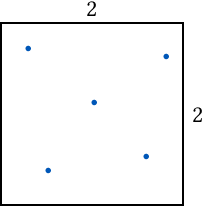
\includegraphics[width=\linewidth]{Images/image-2.png}}
\begin{proof}
    Divide square into 4 smaller squares. We now have 4 pigeonholes and 5 dots:
    \begin{figure}[H]
        \centering
        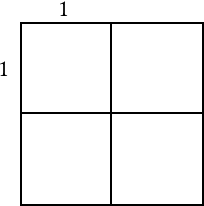
\includegraphics[width=100pt]{Images/image-3.png}
    \end{figure}
    These two points in the same pigeonhole have distance $\leq \sqrt{1^2+1^2}=\sqrt{2}$.
\end{proof}

\eg There exists two people in NYC who have exactly the same number of hairs on their head.

\eg There are 30 people at a party talking with each other. Afterwards, there will be two people who talked with the same number of people.
\begin{proof}
    If we put a person who talked to $i$ people into box $i$, we get 30 boxes; however, we cannot have someone who talked to 0 people and someone who talked at 29 people at the same time! Hence, we combine the box 0 and box 29, and only one of which could be the case.

    Now we have 29 boxes and 30 people. By pigeonhole principle, there must be two people who talked with the same amount of people.
\end{proof}

\begin{theorem}[Strong Pigeonhole Principle]
    Given pigeonholes $1,2,\dots,n$ with \uline{capacities} $c_1,c_2,\dots, c_n$ where $c_i\geq 0$; if we have at least $c_1+c_2+\dots+c_n+1$ pigeons in these pigeonholes, then at least one pigeonhole overflows.
\end{theorem}
\begin{proof}
    Suppose BWOC that no pigeonhole overflows. Then for all $i=1,2,\dots,n$, we have the number of pigeons in $i\leq c_i$.

    We add up and get inequalities:\begin{align*}
        \text{total \# pigeons} \leq c_1+c_2+\dots + c_n
    \end{align*}
    Contradiction!
\end{proof}

\eg There are five people supporting two teams. Then at least one team is supported by 3 people.
\begin{proof}
    Assume BWOC that the two teams only have two supporters. Let $c_1=c_2=2$. However, by SPP, $5\geq 2+2+1$, hence one pigeonhole overflows. Therefore, one team must have $>2$ supporters.
\end{proof}

\subsection{B2 First Ramsey Theorem}

There are 6 people taking a class. Then: \begin{itemize}[align=left]
        \item[\underline{either}] there exists 3 people such that each pair of them have previously taken a class together,
        \item[\underline{or (inclusive)}] there exists 3 people such that no two have taken a class together.
    \end{itemize}

\begin{theorem}
    If we have 6 vertices and we draw all edges between them (a $K_6$ graph)\sidenote{$K_6$ stands for \textit{complete graph on 6 vertices.} It has 15 edges.}, then for every possible way of coloring the edges \rt{red} and \bt{blue}, there must exist a \textbf{monochromatic} triangle.

    \[\begin{tikzcd}[ampersand replacement=\&,cramped]
        \& \bullet \\
        \bullet \&\& \bullet \\
        \bullet \&\& \bullet \\
        \& \bullet
        \arrow[color=magenta, no head, from=1-2, to=2-1]
        \arrow[color=magenta, no head, from=1-2, to=2-3]
        \arrow[color=magenta, no head, from=2-3, to=3-3]
        \arrow[color=cyan, no head, from=3-3, to=4-2]
        \arrow[color=magenta, no head, from=4-2, to=3-1]
        \arrow[color=cyan, no head, from=2-1, to=2-3]
        \arrow[color=magenta, no head, from=2-3, to=3-1]
        \arrow[color=cyan, no head, from=3-1, to=2-1]
        \arrow[color=magenta, no head, from=2-1, to=3-3]
        \arrow[color=cyan, no head, from=3-3, to=3-1]
        \arrow[color=magenta, no head, from=1-2, to=4-2]
        \arrow[color=magenta, no head, from=2-1, to=4-2]
        \arrow[color=cyan, no head, from=4-2, to=2-3]
        \arrow[color=cyan, no head, from=1-2, to=3-3]
        \arrow[color=cyan, no head, from=1-2, to=3-1]
    \end{tikzcd}\]
\end{theorem}
\begin{proof}
    \hypertarget{k6k3k3}{Pick} any vertex and call it $A$. It has 5 edges colored \rt{red} and \bt{blue}. By the SPP, there exists at least 3 edges of the same color. WLOG let these three edges be \rt{red} and call the other three vertices $B,C,D$.
    \[\begin{tikzcd}[ampersand replacement=\&,cramped]
        \&\& {\bullet B} \\
        {A\,\bullet} \&\&\& {\bullet C} \\
        \&\& {\bullet D}
        \arrow[color=magenta, no head, from=2-1, to=1-3]
        \arrow[color=magenta, no head, from=2-1, to=2-4]
        \arrow[color=magenta, no head, from=2-1, to=3-3]
        \arrow[dashed, no head, from=1-3, to=2-4]
        \arrow[dashed, no head, from=3-3, to=2-4]
        \arrow[dashed, no head, from=1-3, to=3-3]
    \end{tikzcd}\]
    \begin{itemize}
        \item If $BC$ is \rt{red}, then $ABC$ is a \rt{red} triangle.
        \item If $CD$ is \rt{red}, then $ACD$ is a \rt{red} triangle.
        \item If $BD$ is \rt{red}, then $ABD$ is a \rt{red} triangle.
        \item If none of the above has happened, then $BC,CD,BD$ are all \bt{blue}, meaning that $BCD$ is a \bt{blue} triangle!
    \end{itemize}
\end{proof}

\begin{theorem}
    If there are 5 instead of 6 vertices, then the above coloring prediction cannot be made with certainty.
\end{theorem}
\begin{proof}[Counterexample]
    \[\begin{tikzcd}[ampersand replacement=\&,cramped,column sep=tiny]
        \&\& \bullet \\
        \bullet \&\&\&\& \bullet \\
        \& \bullet \&\& \bullet
        \arrow[color=magenta, no head, from=1-3, to=2-1]
        \arrow[color=cyan, no head, from=2-1, to=2-5]
        \arrow[color=magenta, no head, from=1-3, to=2-5]
        \arrow[color=cyan, no head, from=1-3, to=3-2]
        \arrow[color=cyan, no head, from=1-3, to=3-4]
        \arrow[color=magenta, no head, from=2-1, to=3-2]
        \arrow[color=magenta, no head, from=3-2, to=3-4]
        \arrow[color=magenta, no head, from=3-4, to=2-5]
        \arrow[color=cyan, no head, from=3-2, to=2-5]
        \arrow[color=cyan, no head, from=2-1, to=3-4]
    \end{tikzcd}\]
\end{proof}


\subsection{B3 $K_p\to K_q,\, K_r$}

In graphy theory, $K_n$ is the \textbf{complete} graph on $n$ vertices.
\begin{table}[H]
    \centering
    \begin{tabular}{lcll}
        $K_1$ &$\bullet$& 1 vertex & 0 edges\\
        $K_2$ &\begin{tikzcd}[ampersand replacement=\&,cramped]
            \bullet \& \bullet
            \arrow[no head, from=1-1, to=1-2]
        \end{tikzcd}& 2 vertices & 1 edge\\[0.1in]
        $K_3$ &\begin{tikzcd}[ampersand replacement=\&,cramped,column sep=3pt,row sep=scriptsize]
            \& \bullet \\
            \bullet \&\& \bullet
            \arrow[no head, from=1-2, to=2-1]
            \arrow[no head, from=1-2, to=2-3]
            \arrow[no head, from=2-1, to=2-3]
        \end{tikzcd}& 3 vertices & 3 edges\\[0.3in]
        $K_4$ &\begin{tikzcd}[ampersand replacement=\&,cramped,sep=scriptsize]
            \bullet \& \bullet \\
            \bullet \& \bullet
            \arrow[no head, from=1-1, to=1-2]
            \arrow[no head, from=1-1, to=2-1]
            \arrow[no head, from=2-1, to=2-2]
            \arrow[no head, from=1-2, to=2-2]
            \arrow[no head, from=2-1, to=1-2]
            \arrow[no head, from=1-1, to=2-2]
        \end{tikzcd}& 4 vertices & 6 edges\\[0.3in]
        $K_5$ &\begin{tikzcd}[ampersand replacement=\&,cramped,column sep=1.5pt, row sep=13pt]
            \&\& \bullet \\
            \bullet \&\&\&\& \bullet \\
            \& \bullet \&\& \bullet
            \arrow[color=magenta, no head, from=1-3, to=2-1]
            \arrow[color=cyan, no head, from=2-1, to=2-5]
            \arrow[color=magenta, no head, from=1-3, to=2-5]
            \arrow[color=cyan, no head, from=1-3, to=3-2]
            \arrow[color=cyan, no head, from=1-3, to=3-4]
            \arrow[color=magenta, no head, from=2-1, to=3-2]
            \arrow[color=magenta, no head, from=3-2, to=3-4]
            \arrow[color=magenta, no head, from=3-4, to=2-5]
            \arrow[color=cyan, no head, from=3-2, to=2-5]
            \arrow[color=cyan, no head, from=2-1, to=3-4]
        \end{tikzcd}& 5 vertices & 10 edges\\[0.4in]
        $K_6$ &\begin{tikzcd}[ampersand replacement=\&,cramped,column sep=12pt, row sep=8pt]
            \& \bullet \\
            \bullet \&\& \bullet \\
            \bullet \&\& \bullet \\
            \& \bullet
            \arrow[color=magenta, no head, from=1-2, to=2-1]
            \arrow[color=magenta, no head, from=1-2, to=2-3]
            \arrow[color=magenta, no head, from=2-3, to=3-3]
            \arrow[color=cyan, no head, from=3-3, to=4-2]
            \arrow[color=magenta, no head, from=4-2, to=3-1]
            \arrow[color=cyan, no head, from=2-1, to=2-3]
            \arrow[color=magenta, no head, from=2-3, to=3-1]
            \arrow[color=cyan, no head, from=3-1, to=2-1]
            \arrow[color=magenta, no head, from=2-1, to=3-3]
            \arrow[color=cyan, no head, from=3-3, to=3-1]
            \arrow[color=magenta, no head, from=1-2, to=4-2]
            \arrow[color=magenta, no head, from=2-1, to=4-2]
            \arrow[color=cyan, no head, from=4-2, to=2-3]
            \arrow[color=cyan, no head, from=1-2, to=3-3]
            \arrow[color=cyan, no head, from=1-2, to=3-1]
        \end{tikzcd}& 6 vertices & 15 edges\\
    \end{tabular}
\end{table}
\rmk Note that $K_n$ has $1+2+3+\dots+(n-1)=\frac{n(n-1)}{2}$ edges, hence is the $n-1$-th triangular number.

Ramsey Theory uses the following language convention: the expression \begin{align*}
    K_p\to K_q,\, K_r
\end{align*}
represents a statement with the following meaning:

\defn If the edges of $K_p$ are colored \rt{red}/\bt{blue}, then it necessarily follows that either the $K_p$ contains a \rt{red $K_q$}, or $K_p$ contains a \bt{blue $K_r$} (or possibly both).

We want to know whether this statement is true for a given triple of $(p,q,r)$.

\eg We proved in  \hyperlink{k6k3k3}{\textbf{B2}} that $K_6\to K_3, K_3$.

\noneg We also showed that $K_5\to K_3,K_3$ is false \sidenote{write $K_5\not\to K_3,K_3$}by exhibiting a coloring of $K_5$ that does not have a red or blue triangle (counterexample).

\eg It is known that $K_{18}\to K_4, K_4$ and $K_{17}\not \to K_4,K_4$.

\eg Also, $K_9\to K_3,K_4$ and $K_8\not \to K_3,K_4$.\sidenote{Here we have to decide in advance which color goes with the $K_3$ and which goes with the $K_4$ due to asymmetry.}
\[\begin{tikzcd}[ampersand replacement=\&,cramped,row sep=26pt]
	\& \bullet \& \bullet \\
	\bullet \&\&\& \bullet \\
	\bullet \&\&\& \bullet \\
	\& \bullet \& \bullet
	\arrow[color=magenta, no head, from=1-2, to=2-1]
	\arrow[color=magenta, no head, from=1-3, to=1-2]
	\arrow[color=magenta, no head, from=2-4, to=1-3]
	\arrow[color=magenta, no head, from=3-4, to=2-4]
	\arrow[color=magenta, no head, from=4-3, to=3-4]
	\arrow[color=magenta, no head, from=4-2, to=4-3]
	\arrow[color=magenta, no head, from=3-1, to=4-2]
	\arrow[color=magenta, no head, from=2-1, to=3-1]
	\arrow[color=cyan, no head, from=2-4, to=1-2]
	\arrow[color=cyan, no head, from=3-4, to=1-2]
	\arrow[color=magenta, no head, from=4-3, to=1-2]
	\arrow[color=cyan, no head, from=4-2, to=1-2]
	\arrow[color=cyan, no head, from=3-1, to=1-2]
	\arrow[color=cyan, no head, from=2-1, to=1-3]
	\arrow[color=cyan, no head, from=3-1, to=1-3]
	\arrow[color=magenta, no head, from=4-2, to=1-3]
	\arrow[color=cyan, no head, from=4-3, to=1-3]
	\arrow[color=cyan, no head, from=3-4, to=1-3]
	\arrow[color=cyan, no head, from=2-1, to=2-4]
	\arrow[color=magenta, no head, from=3-1, to=2-4]
	\arrow[color=cyan, no head, from=4-2, to=2-4]
	\arrow[color=cyan, no head, from=4-3, to=2-4]
	\arrow[color=magenta, no head, from=2-1, to=3-4]
	\arrow[color=cyan, no head, from=3-1, to=3-4]
	\arrow[color=cyan, no head, from=4-2, to=3-4]
	\arrow[color=cyan, no head, from=3-1, to=4-3]
	\arrow[color=cyan, no head, from=2-1, to=4-3]
\end{tikzcd}
\]
\[\text{This $K_8$ has no red triangle and no blue }K_4.\]

\addlink{Ramsey's theorem}
\theorem[Ramsey] Let $q,r$ be positive integers. Then there always exists a positive integer $p$ such that \[K_p\to K_q,K_r\] is true.

We would see the following tabel giving us values of $p$ that work.

Define a function $N(q,r)$ recursively: \sidenote{$q,r\in \Z^+$}
\begin{itemize}
    \item Base case: $N(1,r)=N(q,1)=1$
    \item Recurrence: $N(q,r)=N(q-1,r)+N(q,r-1)$ if $q,r\geq 2$.
\end{itemize}
\hypertarget{tableforN}{}
We compute the value of $N(q,r)$ for:\sidenote{They do look like simplex numbers!}
\begin{table}[H]
    \centering
    \begin{tabular}{lcccccc}
    $q\backslash r$ & 1 & 2 & 3  & 4  & 5   & 6   \\
    1                  & 1 & 1 & 1  & 1  & 1   & 1   \\
    2                  & 1 & 2 & 3  & 4  & 5   & 6   \\
    3                  & 1 & 3 & 6  & 10 & 15  & 21  \\
    4                  & 1 & 4 & 10 & 20 & 35  & 56  \\
    5                  & 1 & 5 & 15 & 35 & 70  & 126 \\
    6                  & 1 & 6 & 21 & 56 & 126 & 252
    \end{tabular}
\end{table}
We would want to prove that $K_{N(q,r)}\to K_q,K_r$ for all $q,r\geq 1$.
\begin{proof}
    By induction.
    \begin{enumerate}[align=left]
        \item[\textit{Base case}:] \begin{tabular}[t]{rl}
            If $q=r=1$, then $N=1$, we need to show that& $K_1\to K_1,K-r$\\
            and & $K_1\to K_q,K_1$
        \end{tabular} for all $q,r$. 
        
        That is, suppose $K_1$ has its edges colored \rt{red}/\bt{blue}, then there exists a \rt{red $K_1$} or a \bt{blue $K_r$}, and \textit{vice versa}. 
        
        Since there are no edges, this is vacuously true.

        \item[\textit{Inductive step}:] \hypertarget{ramseyInductive}{We} will show\sidenote{This works because as we fill out the table above, each new number we write in will work because it's the sum of the left and above numbers and they both work.} 
        that \uline{if we are given that} $A,B$ are numbers such that \begin{align*}
            K_A&\to K_{q-1},K_r\\
            \text{and }K_B&\to K_q, K_{r-1}
        \end{align*}
        are true, \uline{then} $K_{A+B}\to K_q,K_r$.

        Consider $K_{A+B}$ colored \rt{red} and \bt{blue}. We will show that it has a \rt{red $K_q$} or a \bt{blue $K_r$}.
        
        Pick a vertex and call it $X$. It would have $A+B-1$ edges in total. We claim that \dashuline{$X$ either has at least $A$ \rt{red} edges, or at least $B$ \bt{blue} edges}. This is indeed true, because if not, the number of \rt{red} edges would be $\leq A-1$ and the number of \bt{blue} edges would be $\leq B-1$ and so the total number of edges would be $\leq A+B-2<A+B-1$, which is a contradiction.

        Now, if $X$ has a \rt{red claw} of size $A$:\sidenote{The neighbouring vertices connected by black edges form $K_A$, yet to be colored.}
        \[\begin{tikzcd}[ampersand replacement=\&,cramped]
            X \&\& \dots \& {K_A} \\
            \&\& \bullet \\
            \dots \& \bullet
            \arrow[color=magenta, dashed, no head, from=1-1, to=1-3]
            \arrow[color=magenta, no head, from=1-1, to=2-3]
            \arrow[color=magenta, no head, from=1-1, to=3-2]
            \arrow[color=magenta, dashed, no head, from=1-1, to=3-1]
            \arrow[no head, from=1-3, to=2-3]
            \arrow[no head, from=1-3, to=3-2]
            \arrow[no head, from=2-3, to=3-2]
            \arrow[no head, from=3-1, to=3-2]
            \arrow[no head, from=3-1, to=2-3]
        \end{tikzcd}\]
        From our inductive hypothesis $K_A\to K_{q-1},K_r$, we must have \begin{itemize}[align=left]
            \item[\textbf{either}] \rt{red $K_{q-1}$}, in which case we combine with the vertex $X$ and the red claw to get at least one \rt{red $K_q$}.
            \item[\textbf{or}] \bt{blue $K_r$}, in which case we are done. 
        \end{itemize}
        Similarly, if $X$ has a \bt{blue claw} of size $B$, then we make the same argument.
        \vspace{0.2in}
        
        Hence, we know that $K_{A+B}\to K_q,K_r$ is true whenever $K_A\to K_{q-1},K_r$ and $K_B\to K_{q},K_{r-1}$.
    \end{enumerate}
\end{proof}

\subsection{B4 Ramsey numbers}
Recall: Let $m,n$ be positive integers. We know that there are numbers $p\in \N$ such that $K_p\to K_m,K_n$.

\rmk If $p$ works, then so does any $q\geq p$ as $K_q$ would contain copies of $K_p$.

So the question becomes, if we have $K_p\to K_m,K_n$, is $p$ the \textbf{smallest} such number?

\defn The \textbf{Ramsey number} $r(m,n)$ is the smallest such number.

\eg We know $K_6\to K_3,K_3$ but $K_5\not\to K_3,K_3$, so $r(3,3)=6$.

\eg Mathematicians have proved that \begin{align*}
    K_{48} &\to K_5,K_5\\
    K_{42} &\not\to K_5,K_5
\end{align*}
so we have $43\leq r(5,5)\leq 48$.

\rmk In general, \begin{align*}
    K_N&\to K_m, K_n \iff r(m,n)\leq N\\
    K_{N-1} &\not\to K_m,K_n \iff r(m,n)\geq N
\end{align*}
Need both to get the precise value of $r(m,n)$.

\begin{proposition} Properties of Ramsey numbers:
\begin{enumerate}[label=(\alph*)]
    \item $r(3,3)=6$ \sidenote{proven in  \hyperlink{k6k3k3}{\textbf{B2}}}
    \item $r(m,n) = r(n,m)$\sidenote{symmetry}
    \item $r(1,n)=1$\sidenote{$K_1\to K_1,K_n$, $K_0\not\to K_1,K_n$}
    \item $r(2,n)=n$
    \item $r(m,n)\leq r(m-1,n)+r(m,n-1)$ for all $m,n\geq2$
\end{enumerate}
\begin{proof}[Proof for (d)]
    Claim: $K_2\to K_2,K_n$, $K_{n-1}\not\to K_2,K_n$.
    
    Color $K_n$. If all edges are blue then we have a \bt{blue $K_n$}. Else we have some red edges, so we have some \rt{red $K_2$}.

    Now color $K_{n-1}$ all blue: we realize that we don't have any red $K_2$, but we don't have a blue $K_n$ either!
\end{proof}
\begin{proof}[Proof for (e)]
    Let $A=r(m-1,n)$, $B=r(m,n-1)$. We have shown that if $K_A\to K_{m-1},K_n$ and $K_B\to K_{m},K_{n-1}$, then $K_{A+B}\to K_m, K_n$. Hence $r(m,n)\leq A+B$.
\end{proof}
\end{proposition}

Known facts:
\begin{align*}
    r(2,2) &=2\\
    r(3,3) &=6\\
    r(4,4) &=18\\
    43\leq r(5,5)&\leq 48\\
    102\leq r(6,6)&\leq 165
\end{align*}

\subsection{B5 A lower bound for $r(m,n)$}
Our \hyperlink{tableforN}{table of $N(m,n)$} gave us upper bonds for $r(m,n)$. Specifically, \begin{align*}
    r(m,n)\leq N(m,n)=\frac{(n+m-2)!}{(n-1)!(m-1)!}=
   {{m+n-2}\choose{m-1}}
\end{align*}

What about lower bound?

\begin{theorem}
    \begin{align*}
        r(m,n)\geq (m-1)(n-1)+1
    \end{align*}
    \ifnif $K_{(m-1)(n-1)}\not\to K_m, K_n$
\end{theorem}

\begin{proof}
    We prove this by exhibiting a coloring of $K_{(m-1)(n-1)}$ that has no red $K_m$, no blue $K_n$.
    
    Place vertices in grid:
    \[\begin{tikzcd}[ampersand replacement=\&,cramped,sep=small]
        \bullet \& \bullet \& \dots \& \bullet \\
        \bullet \& \bullet \& \dots \& \bullet \\
        \vdots \& \vdots \& \ddots \& \vdots \\
        \bullet \& \bullet \& \dots \& \bullet
        \arrow["{m-1\text{ rows}}"', shift right=4, draw=none, from=1-1, to=4-1]
        \arrow["{n-1\text{ columns}}"', shift right=5, draw=none, from=4-1, to=4-4]
    \end{tikzcd}\]
    Coloring rule of edges: If two vertices are in the same row, color the edges \bt{blue}. If two vertices are in the same column, color the edges \rt{red}. Every other edge arbitrary.

    Claim: there exists no \rt{red} $K_m$.

    Consider the $m$ vertices of such a $K_m$. There are $m-1$ rows. Pigeonhole principle ensures that some vertices must be in the same row. But that edge must be \bt{blue}! So this is not a red $K_m$. Similarly, there are no blue $K_n$.
\end{proof}

Thus, we get: $\displaystyle (m-1)(n-1)+1\leq r(m,n)\leq \frac{(n+m-2)!}{(n-1)!(m-1)!}=
{{m+n-2}\choose{m-1}}$.

Observe there is still a huge gap between the bounds. Could we get better?

\subsection{B6 The ``parity'' improvement}
Our methods have shown that $K_{10}\to K_3,K_4$. But it is actually true that $K_{9}\to K_3,K_4$. Why?
\begin{proof}
    Given $K_9$ colored red or blue. We seek a \rt{red $K_3$} or a \bt{blue $K_4$}. 
    
    That is to say that if we ever see a \rt{red 4-claw}, then we are done!\sidenote{See \hyperlink{k6k3k3}{this} argument.}
    \[\begin{tikzcd}[ampersand replacement=\&,cramped]
        \bullet \&\& \bullet \\
        \&\& \bullet \\
        \& \bullet \& \bullet
        \arrow[color=magenta, no head, from=1-1, to=1-3]
        \arrow[color=magenta, no head, from=1-1, to=3-3]
        \arrow[color=magenta, no head, from=1-1, to=2-3]
        \arrow[color=magenta, no head, from=1-1, to=3-2]
    \end{tikzcd}\]

    In addition, if we ever see a \bt{blue 6-claw}, then we are also done because $K_6\to K_3,K_3$ and we either have a \rt{red $K_3$} or a \bt{blue $K_3$}, which would have to combine with the other vertex to get a blue $K_4$.

    Now suppose we neither have a red 4-claw nor a blue 6-claw. This implies that each vertex has $\leq 3$ \rt{red} edges, and $\leq 5$ blue edges. However, in a $K_9$, \dashuline{each vertex only has 8 edges}, so they must \dashuline{exactly each have 3 red edges and 5 blue edges}. Does this exist? We realize that to make this happen, we have:\begin{itemize}
        \item 9 vertices
        \item Each vertex has 3 red edges
        \item Every edge belongs to two vertices
    \end{itemize}
    Hence, we need to have exactly $\frac{3\times9}{2}=13.5$ red edges, but this cannot happen because we need a whole number of edges! Thus, it is not possible that we neither have a red 4-claw nor a blue 6-claw.
\end{proof}

\begin{lemma}[Ramsey inductive step improved by parity]
    Suppose\sidenote{Also seen \hyperlink{ramseyInductive}{here}.} \begin{align*}
        K_A&\to K_{q-1},K_r\\
        \text{and }K_B&\to K_q, K_{r-1}
    \end{align*}
    are true, \uline{then} $K_{A+B}\to K_q,K_r$.

    In addition, if $A,B$ are \textbf{both even numbers}, then $K_{A+B-1}\to K_q,K_r$.
\end{lemma}

\subsection{B7 Variations}
\subsubsection{\rt{More }\gt{colors}\bt{!} }

For example:\begin{align*}
    K_p\to K_a,K_b,K_c
\end{align*}
(given $K_p$ colored \rt{red}, \bt{blue}, \gt{green}, it must contain a red $K_a$, or a blue $K_b$, or a green $K_c$.)

\eg It is known that $K_{17}\to K_3,K_3,K_3$.
\begin{proof}[Proof sketch]
    Pick a vertex which has 16 edges. We observe $16\div 3=5\frac{1}{3} \implies $ at least one color occurs 6 times (i.e. we can see a red/blue/green 6-claws).
\end{proof}

\rmk $r(a,b,c)$ is the smallest number that works for the above.

\subsubsection{Other graphs}
\begin{itemize}[align=left]
    \item[Paths: ] \[\begin{tikzcd}[ampersand replacement=\&,cramped,sep=small]
        {P_1} \& \bullet \\
        {P_2} \& \bullet \& \bullet \\
        {P_3} \& \bullet \& \bullet \& \bullet \\
        {P_4} \& \bullet \& \bullet \& \bullet \& \bullet
        \arrow[no head, from=2-2, to=2-3]
        \arrow[no head, from=3-2, to=3-3]
        \arrow[no head, from=3-3, to=3-4]
        \arrow[no head, from=4-2, to=4-3]
        \arrow[no head, from=4-3, to=4-4]
        \arrow[no head, from=4-4, to=4-5]
    \end{tikzcd}\]
    \item[Claws: ]  \[\begin{tikzcd}[ampersand replacement=\&,cramped,column sep=small,row sep=tiny]
        {K_{1,1}} \& \bullet \& \bullet \& {K_{1,4}} \& \bullet \& \bullet \\
        {K_{1,2}} \& \bullet \& \bullet \&\&\& \bullet \\
        \&\& \bullet \&\&\& \bullet \\
        {K_{1,3}} \& \bullet \& \bullet \&\&\& \bullet \\
        \&\& \bullet \\
        \&\& \bullet
        \arrow[no head, from=1-2, to=1-3]
        \arrow[no head, from=2-2, to=2-3]
        \arrow[no head, from=2-2, to=3-3]
        \arrow[no head, from=4-2, to=4-3]
        \arrow[no head, from=5-3, to=4-2]
        \arrow[no head, from=6-3, to=4-2]
        \arrow[no head, from=1-5, to=1-6]
        \arrow[no head, from=2-6, to=1-5]
        \arrow[no head, from=3-6, to=1-5]
        \arrow[no head, from=4-6, to=1-5]
    \end{tikzcd}\]
\end{itemize}

\eg Show that $r(K_{1,3}, K_{1,3}) = 6$.
\begin{proof}
    We know $K_6\to K_3,K_3$. Pick a vertex that has 5 neighbors. By the strong pigeonhole principle, we must have three edges of the same color $\implies$ either red or blue $K_{1,3}$.
\end{proof}

\section{C Counting}
\subsection{C1 Three principles}
\subsubsection{Addition principle}\sidenote{aka. counting by cases}
\defn If a set $S$ is \textit{partitioned}\sidenote{that is, $S=\bigcup S_i$ and $S_i\cap S_j=\emptyset$ whenever $i\neq j$} into subsets $S_1,S_2,\dots S_n$, then the cardinality of $S$ is $$|S|=|S_1|+\dots +|S_n|.$$

The art lies in:\begin{itemize}
    \item making each $S_i$ easy to count, and
    \item not having too many $S_i$ if there is no formula for $|S_i|$.
\end{itemize}

\rmk[Variations] If the $S_i$ cover $S$ but they overlap\sidenote{The inclusion/exclusion principle handles overlaps precisely}, then we have the inequality $\displaystyle |S|<\sum_{i=1}^{n}|S_i|$ because the overlap implies that we are \textit{overcounting}.

\eg Let $S$ be the set of \textit{good}\sidenote{\textit{good} meaning no adjacent elements} subsets of $[5]=\{1,2,3,4,5\}$. We could first try:\begin{itemize}
    \item $S_1$ contains the subsets that contain 5
    \item $S_2$ contains the subsets that don't contain 5
\end{itemize}
We have previously shown that $|S_1|=$ number of \textit{good} subsets of [3] and $|S_2|=$ number of \textit{good} subsets of [4].

Alternatively, we could also let $T_i$ be the \textit{good} subsets of $[5]$ with cardinality $i$. Then $S$ is \uline{partitioned} into $T_0\cup T_1\cup T_2\cup T_3$. We count:
\[\begin{tikzcd}[ampersand replacement=\&,cramped]
	{T_0:} \& \emptyset \& {|T_0|=1} \\
	{T_1:} \& {1,2,3,4,5} \& {|T_1|=5} \\
	{T_2:} \& {13,14,15,24,25,35} \& {|T_2|=6} \\
	{T_3:} \& 135 \& {|T_3|=1}
	\arrow["{|S|=13}", shift left=5, bend left=40, no head, from=1-3, to=4-3]
\end{tikzcd}\]

\subsubsection{Subtraction principle}
\defn Let $A\subseteq S$ and $A^c$ be its complement in $S$. Then $A, A^c$ partition $S$ and $|S|=|A|+|A^c|$. This means that $$|A|=|S|-|A^c|.$$

\eg How many 2-digit numbers have distinct nonzero digits?

Let $S$ be the set of all 2-digit numbers $\{10,11,\dots,99\}$ and let $A$ be the subset of those with nonzero distinct digits. We count:\begin{align*}
    A^c: &11,22,\dots,99 &&\text{(distinct fails)}\\
    &10,20,\dots, 90 &&\text{(nonzero fails)}
\end{align*}
Hence $|A|=|S|-|A^c|=90-18=72$.

\subsubsection{Multiplication principle}
\defn Suppose we have to do two tasks in sequence\sidenote{Note: sometimes the 2nd task could depend on the 1st one}. We suppose:\begin{itemize}
    \item Task 1 has $m$ outcomes
    \item Task 2 has $n$ outcomes, regardless of how Task 1 was carried out.
\end{itemize}
Then there are $mn$ ways of carrying out both tasks.\sidenote{Similarly for 3 or more tasks in sequence}

\eg How many 2-digit numbers have distinct nonzero digits?

Let \circled{a}\circled{b} be the two digits in these numbers. Let Task 1 be selecting digit \circled{a} and Task 2 be selecting digit \circled{b}.\begin{itemize}
    \item Task 1: 9 ways (1,2,\dots,9)
    \item Task 2: 8 ways (1,2\dots,9 but not same as \circled{a})
\end{itemize}
Hence there are $9\times 8=72$ such numbers.

\cautiouseg How many \textbf{odd} numbers in the range 1000-9999 have distinct digits?
\begin{itemize}[align=left]
    \item[\textbf{Attempt 1}:] Let \circled{a}\circled{b}\circled{c}\circled{d} be the 4 digits in these numbers and assign them Tasks 1-4. We have: \begin{itemize}
        \item Task 1: 9 ways (1-9)
        \item Task 2: 9 ways (0-9 except \circled{a})
        \item Task 3: 8 ways (0-9 except \circled{a},\circled{b})
        \item \rt{Task 4}: Could be 2 or 3 or 4 or 5 (depending on how many odd digits had already been used)
    \end{itemize}
    Hence, the best we can say\sidenote{BAD! This is a large range!} here is that the answer is between $9\times9\times8\times2$ and $9\times9\times8\times5$.

    \item[\textbf{Attempt 2}:] Let \circled{a}\circled{b}\circled{c}\circled{d} be the 4 digits in these numbers and try the order \circled{d}\circled{a}\circled{b}\circled{c} for Tasks 1-4. We have: \begin{itemize}
        \item Task 1: 5 ways $(1,3,5,7,9)$
        \item Task 2: 8 ways (1-9 except \circled{d})
        \item Task 3: 8 ways (0-9 except \circled{a}, \circled{d})
        \item Task 4: 7 ways (0-9 except \circled{a}, \circled{d}, \circled{b})
    \end{itemize}
    Therefore, the number of ways is $5\times 8\times 8\times 7=2240$.
\end{itemize}

\eg How many numebrs $0,1,\dots 99999$ have exactly one digit 6?

We can assign tasks:\begin{itemize}
    \item Task 1: choose a location for 6, giving us 5 ways
    \item Task 2: assign the remaining digits from left to right, giving us $9^4$ ways
\end{itemize}

Hence there are $5\times 9^4=32805$ such numbers.

\noneg How many integers $0,1,\dots 99999$ have \textit{at least} one digit 6?

\textbf{Attempt:} We can assign tasks:\begin{itemize}
    \item Task 1: choose a location for 6, giving us 5 ways
    \item Task 2: assign the remaining digits from left to right, giving us $10^4$ ways
\end{itemize}

But the answer of 50000 is \rt{\textbf{wrong}}! But why?

The counting process for this problem is corresponding the ways of performing tasks to valid 5-digit numbers:
\drawing{0.6\linewidth}{image-4.png}
We have correctly counting the \gt{green} set. However, for this to count the \bt{blue} set, we need $f$ to be \textbf{bijective}. That is, every valid number must be obtained in exactly one way. However, in this case, our $f$ is surjective but not injective. For instance, 62516 will be counted \textit{twice}:\begin{itemize}
    \item 6\_\_\_\_ then 62516; or
    \item \_\_\_\_6 then 62516.
\end{itemize}
Hence, 50000 > correct answer!

\textbf{Correct way:} Using the subtract principle to deduct numbers that don't have 6: $10^5-9^5=40951<50000$.

\subsection{C2 Probability}
\defn \begin{align*}
    \text{Probability} = \frac{\text{number of favourable cases}}{\text{number of total cases}}
\end{align*}

\eg Probability of 3 dice rolling the same number: $P=\frac{6}{6^3}=\frac{1}{36}$.

\subsection{C3 The counting framework}
Here is a very general problem:

``How many distinguishable ways to map a multiset $S$ to a multiset $T$ satisfying given constraints?''

\eg There are fruits and plates. Let $S=\{3\cdot \text{apple}, 1\cdot \text{banana}\}$ and $T=\{2\cdot \text{circle}, 1\cdot \text{rectangle}\}$. How many ways are there to serve fruit on plates such that the rectangular plate has an even number of fruit?
\drawing{0.6\linewidth}{image-5.png}

\textbf{Ans:} Organize by number of fruit on rectangle.
\drawing{0.6\linewidth}{image-6.png}
\drawing{0.6\linewidth}{image-7.png}
\drawing{0.6\linewidth}{image-8.png}

Hence there are 9 ways.

\subsubsection{The general counting problem}
Let there be multisets \begin{align*}
    S&=\{a_1\cdot 1, a_2\cdot2, \dots, a_s\cdot s\} &\text{object types }1,2,\dots,s\\
    T&=\{b_1\cdot U_1, b_2\cdot U_2,\dots,b_t\cdot U_t\} &\text{box types }U_1,\dots,U_t\\
\end{align*}
How many distinguishable maps $f: S\to T$ are there, subject to restrictions on the numbers $u_i=\left|\inv{f}(U_i)\right|$?\sidenote{The number of items mapped to boxes of type $U_i$}

\rmk[Special cases] To recognize which situation applies to the problem:
\begin{itemize}
    \item By objects:\begin{itemize}
        \item Distinct: $S=\{1,2,\dots,s\}$
        \item Identical: $S=\{s\cdot 1\}$
    \end{itemize}
    \item By boxes: \begin{itemize}
        \item Distinct: $T=\{U_1,\dots, U_t\}$
        \item Identical: $T=\{t\cdot U_1\}$
    \end{itemize}
    \item For each case above, we can apply constraints:\begin{itemize}
        \item $0\leq u_i\leq 1$
        \item $0\leq u_i<\infty$\qquad{no constraint}
        \item $1\leq u_i<\infty$\qquad{nonempty}
        \item $0\leq u_i\leq n_i$ for some $n_i\in \N_0$\qquad{max. capacity}
        \item $u_i\in N_i\subseteq \N$
    \end{itemize}
\end{itemize}
\drawing{0.95\linewidth}{table3-1.pdf}

\eg We have 10 distinct books to be shared between 2 children. Each child needs 2 books to avoid a crisis.\sidenote{Table entry \circled{15}}
\begin{itemize}
    \item Distinct objects $\{1,2,\dots,10\}$
    \item Distinct boxes $\{U_1,U_2\}$
    \item Constraints: $u_i\in [2,\infty[$
\end{itemize}

\eg[Attempt 1] 10 distinct books, 5 of them to be arranged on shelf (order matters)\sidenote{Table entry \circled{15}}
\begin{itemize}
    \item $S=\{1,2,\dots,10\}$
    \item $T=\{U_1,U_2,\dots,U_5, \rt{U_6}\}$ (positions on shelf + extra for unshelved books)
    \item $u_1=\dots=u_5=1, u_6=5$
\end{itemize}

\eg[Attempt 2] 10 distinct books, 5 of them to be arranged on shelf (order matters)\sidenote{Table entry \circled{1}, easier!}
\begin{itemize}
    \item $S=\{1,2,\dots,5\}$ (numbered stickers to arrange books)
    \item $T=\{U_1,U_2,\dots,U_{10}\}$ (10 books)
    \item $0\leq u_1\leq 1$ (each book can get 0 or 1 sticker)
\end{itemize}

\eg I have 10 books and will take 5 on holiday.
\begin{itemize}
    \item Take 1:\sidenote{Table entry \circled{15}} \begin{itemize}
        \item $S=\{1,2,\dots,10\}$
        \item $T=\{U_1,U_2\}$
        \item $u_1=u_2=5$
    \end{itemize}
    \item Take 2:\sidenote{Table entry \circled{2}} \begin{itemize}
        \item $S=\{5\cdot 1\}$ (identical `stickers' marking on-holiday)
        \item $T=\{U_1,U_2\,\dots,U_{10}\}$
        \item $0\leq u_1\leq 1$ (each book can get 0 or 1 sticker)
    \end{itemize}
\end{itemize}

\subsection{C4 Permutations of a set}
\rmk Recall $[n]=\{1,2,\dots,n\}$.

\defn Let $0\leq s\leq t$. \begin{itemize}
    \item An \textbf{$s$-permutation} of $[t]$ is an ordered list of $s$ distinct elements of $[t]$.
    \item A \textbf{$t$-permutation} of $[t]$ is just a \textbf{permutation} of $[t]$.
\end{itemize}

\eg 10 books, arrange 5 on shelf: 5-perm of $[10]$
\eg 20 athletes, Gold, Silver and Bronze awarded: 3-perm of [20]

\begin{theorem}
    The number of $s$-perms of $[t]$ is \[\underset{s\text{ terms}}{\underbrace{t(t-1)\dots (t-s+1)}}\]
\end{theorem}
\begin{proof}
    Select elements of the list one-by-one. We have $t$ ways to pick the first, $t-1$ ways of picking the second, etc.
\end{proof}

\defn[$s$-th falling-factorial function] This inspires the following notation \[(x)_s=x(x-1)\dots(x-s+1)=\frac{t!}{(t-s)!}\]\sidenote{There is also a rising $(x)^s=x(x+1)\dots(x+s-1)$}
\rmk $(x)_0=1, (n)_n=n!$

\eg Number of ways to shelve 5 books out of 10 is $$(10)_5=10\times9\times8\times7\times6=30240$$

\subsection{C5 Circular permutations}

A circular 5-perm of $[n]$ is an arrangement of $s$ distinct elements of $[n]$ around a round table. The difference from a non-circular perm is that the orientation of the table does not matter! How many ways to do so?

If there is a head of the table and positions are marked clockwise, then it would be the same as the $s$-perm $(n)_s$.

However, we consider all ways of marking the `head' of the tablen to be equivalent, so we divide $s$ upon that. Hence, we get the answer $\displaystyle\frac{1}{s}(n)_s=\frac{n!}{s(n-s)!}$.

\subsection{C6 Table entries 3,4,5}
\begin{itemize}
    \item \circled{3}: $s$ distinct objects, $t$ identical boxes, 0 or 1 per box.
    \[\# \text{ ways} = \begin{cases}
        1 & s\leq t\\
        0 &\text{otherwise}
    \end{cases}\]
    \item \circled{4}: $s$ identical objects, $t$ identical boxes, 0 or 1 per box.
    \[\# \text{ ways} = \begin{cases}
        1 & s\leq t\\
        0 &\text{otherwise}
    \end{cases}\]
    \item \circled{5}: $s$ distinct objects, $t$ distinct boxes, no restrictions.
    \[\# \text{ ways} = \underset{s \text{ times}}{\underbrace{t\times t\times\dots \times t}}=t^s\]
\end{itemize}

\rmk $0^0=1$ in combinatorics.\sidenote{NOT in analysis!!}

\subsection{C7 Combinations of sets: table entries 2,6,10}
If we let $0\leq s\leq t$, then an \textbf{$s$-combination of} [$t$] is a subset of size $s$ of $[t]$.

\defn The binomial coefficient $t\choose s$ is defined (combinatorially) to be the number of $s$-combinations of $[t]$.

\begin{theorem}
    \[{t\choose s} = \frac{(t)_s}{s!}=\frac{t!}{(t-s)!s!}\]
\end{theorem}
\begin{proof}
    Consider the number of $s$-perms of $[t]$. 
    
    We can count it directly: $(t)_s$.

    Alternatively, make task 1 `selecting a subset of size $s$', which gives us $t\choose s$ ways. Make task 2 the ways of ordering a subset, which give $s!$ ways. By multiplication principle, the number of $s$-perms of $[t]$ is ${t\choose s}s!$.

    We have $(t)_s={t\choose s}s!$, giving us the formula above.
\end{proof}

\eg All of the following are equivalent and satisfy table entry \circled 2\sidenote{$0\leq u_i\leq 1$}:
\begin{itemize}
    \item Select $s$ books out of $t$ distinct books;
    \item Place $s$ stickers on $t$ books, at most one sticker per book;
    \item Put $s$ identical objects into $t$ distinct boxes, each box can only have at most 1 object.
\end{itemize}

\eg These equivalent problems satisfy table entry \circled 6:\sidenote{$0\leq u_i<\infty$}
\begin{itemize}
    \item Solutions to $x_1+x_2+x_3+x_4+x_5=12$ where $x_i\geq 0$ are integers.
    \item Packing a box of 12 bagels of 5 different types of bagels with unlimited supply.
    \item Number of permutations of 12 objects and 4 `drawer dividers': \[\bullet\bullet \,|\, \bullet\bullet\bullet \,|\, \bullet\bullet\,|\, \bullet\bullet\bullet\bullet \,|\, \bullet\]
\end{itemize}

\rmk In general, when we count the number of anagrams $s~\bullet$s and $t-1 \mid$s, there are $s+t-1$ total symbols. We must select $s$ of the $s+t-1$ positions to be $\bullet$. Hence, the number of ways would be\sidenote{LHS is choose $\bullet$, RHS is choose $\mid$.} \[{{s+t-1}\choose s}={{s+t-1}\choose t-1}\]

\eg Entry \circled{10} is the same as \circled 6 except that each box must be nonempty:\begin{itemize}
    \item Solutions to $x_1+\dots + x_s=t$ where $x_i\geq 1$ integers.
    \item Select $s$ bagels from $t$ types, with each type chosen at least once. 
    
    This reduces to the prev problem: select one of each type of bagel first; then, we choose $s-t$ bagels of $t$ types.

    \item Anagrams with $s$ $\bullet$s and $t-1$ $\mid$: must avoid $||$ and $|$ at beginning or end. Then we could think about placing $t-1$ dividers in the $s-1$ spaces between $\bullet$s, giving us $s-1\choose t-1$ ways.
\end{itemize}

\subsection{C8 Anagrams}
\eg Find the number of anagrams of the word \begin{center}
    COMBINATORIALISTICALLY
\end{center}
First, suppose all 22 letters were distinct. We put subscripts:
\[\mathrm{C_1O_1MBI_1NA_1T_1O_2RI_2A_2L_1I_3ST_2I_4C_2A_3L_2L_3Y}\]
Now we have this multiset: \[\{\mathrm{2C, 2O, M, B, 4I, N, 3A, 2T, R, 3L, S, Y}\}\]
We want to find the ways of arranging this!
\begin{itemize}
    \item Assuming everything is distinct: 22! ways.
    \item Same assumption but with two tasks in multiplication:\begin{itemize}
        \item Task 1: Arrange without subscripts (what we want)
        \item Task 2: Add subscripts: the number of ways to add them is \[2!\times 2!\times 1!\times 1!\times 4!\times 1!\times 3!\times 2!\times 1!\times 3!\times 1!\times 1!\]
    \end{itemize}
\end{itemize}
\addlink{Multinomial coefficient}
Therefore, our answer would be (in multinomial coefficient)\sidenote{DO NOT LEAVE OUT 1s}\begin{align*}
    &\frac{22!}{2!\times 2!\times 1!\times 1!\times 4!\times 1!\times 3!\times 2!\times 1!\times 3!\times 1!\times 1!}
    =&{ 22\choose 2,2,1,1,4,1,3,2,1,3,1,1}
\end{align*}

\subsection{C9 More circular tables}
\eg \label[example]{alien-conference} An alien conference has 9 Martian hare delegates and 16 Jovian hare delegates, with each type of hare identical. How many distinguishable ways are there to seat them at a circular table?

Method: first consider the ways of arrangement at a marked table.
\[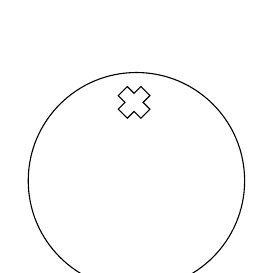
\begin{tikzpicture}[x=0.75pt,y=0.75pt,yscale=-1,xscale=1]
    %uncomment if require: \path (0,300); %set diagram left start at 0, and has height of 300
    
    %Shape: Circle [id:dp9867838680866461] 
    \draw   (77,85.13) .. controls (77,56.34) and (100.34,33) .. (129.13,33) .. controls (157.92,33) and (181.26,56.34) .. (181.26,85.13) .. controls (181.26,113.92) and (157.92,137.26) .. (129.13,137.26) .. controls (100.34,137.26) and (77,113.92) .. (77,85.13) -- cycle ;
    %Shape: Cross [id:dp053203375302823375] 
    \draw   (131.27,39.77) -- (135.62,44.13) -- (132.36,47.39) -- (135.62,50.66) -- (131.27,55.02) -- (128,51.75) -- (124.73,55.02) -- (120.38,50.66) -- (123.64,47.39) -- (120.38,44.13) -- (124.73,39.77) -- (128,43.04) -- cycle ;
    \end{tikzpicture}
    \]

\begin{itemize}
    \item We seat 9 Martian hares and fill out the rest with Jovian ones: $\displaystyle {25\choose 9}$.
    \item We place all hares (the answer we want) and then mark the table. In the end we should get the same answer of $\displaystyle{ 25\choose 9}$.\begin{itemize}
        \item How do we mark the table? There are 25 places that can be marked, but \dashuline{not all of them are distinct}! For instance:
        \[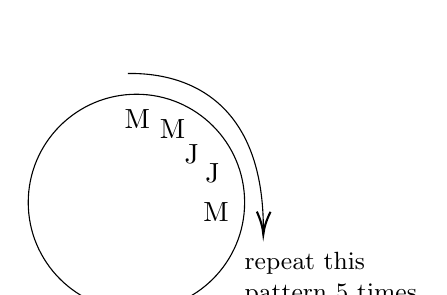
\begin{tikzpicture}[x=0.75pt,y=0.75pt,yscale=-1,xscale=1]
            %uncomment if require: \path (0,300); %set diagram left start at 0, and has height of 300
            
            %Shape: Circle [id:dp9867838680866461] 
            \draw   (77,85.13) .. controls (77,56.34) and (100.34,33) .. (129.13,33) .. controls (157.92,33) and (181.26,56.34) .. (181.26,85.13) .. controls (181.26,113.92) and (157.92,137.26) .. (129.13,137.26) .. controls (100.34,137.26) and (77,113.92) .. (77,85.13) -- cycle ;
            %Curve Lines [id:da9747269900319728] 
            \draw    (125,23) .. controls (156.93,22.53) and (190.58,39.19) .. (190.28,98.71) ;
            \draw [shift={(190.26,100.53)}, rotate = 270.94] [color={rgb, 255:red, 0; green, 0; blue, 0 }  ][line width=0.75]    (10.93,-3.29) .. controls (6.95,-1.4) and (3.31,-0.3) .. (0,0) .. controls (3.31,0.3) and (6.95,1.4) .. (10.93,3.29)   ;
            
            % Text Node
            \draw (122.13,39) node [anchor=north west][inner sep=0.75pt]   [align=left] {M};
            % Text Node
            \draw (139.13,44) node [anchor=north west][inner sep=0.75pt]   [align=left] {M};
            % Text Node
            \draw (151.13,56) node [anchor=north west][inner sep=0.75pt]   [align=left] {J};
            % Text Node
            \draw (161.13,65) node [anchor=north west][inner sep=0.75pt]   [align=left] {J};
            % Text Node
            \draw (160.13,84) node [anchor=north west][inner sep=0.75pt]   [align=left] {M};
            % Text Node
            \draw (180,108) node [anchor=north west][inner sep=0.75pt]  [font=\small] [align=left] {repeat this \\pattern 5 times};
            
            
            \end{tikzpicture}\]
        then the table only has 5 distinct markings due to rotational symmetry.
    \end{itemize}
\end{itemize}
\begin{theorem}
    Consider an arrangement on a circular table with $n$ spots. Let $R_k$ be the action of rotating this table by $k$ places. Define:\sidenote{$F$ is the \textit{stabilizer} of the group action} \[F=\{k\in \Z\mid R_k\text{ leaves the arrangement unchanged}\}\]
    Then we have: \begin{enumerate}
        \item $F$ is the set of multiples of some $d|n$.
        \item A length $d$ pattern would be repeated $\frac{n}{d}$ times (so there are only $\frac{n}{d}$ distinct markings)
    \end{enumerate}
\end{theorem}
\begin{proof}
    Let $d$ be the smallest positive integer such that $R_d\in F$. \sidenote{Review Abstract Alg. 1}
    Suppose BWOC $k\in F$ but $d\not\mid k$. Then let $k=md+r$ with $r\leq d$, and rotation by $r$ would be: $R_kR_{-md}$. Since $k\in F$, this also fixes the arrangement. However, $r<d$ contradicts the fact that $d$ is the smallest positive integer such that $R_d\in F$. 
\end{proof}

Back to \cref{alien-conference}: \(F=d\Z\) where $d=1,5,25$.
\begin{itemize}
    \item If $d=1$, 25 ways of marking the table.
    \item $d=5$, 5 ways of marking.
    \item $d=25$, 1 way of marking.
\end{itemize}

\addlink{Multichoose notation}
\defn[Multichoose notation] Define the ways to select a bag of $k$ items from $n$ different types of item to be $\left({n\choose k}\right) = {k+n-1\choose k}= {k+n-1\choose n-1}$.

\section{D Binomial Coefficients}
We know that $n\choose k$ is the number of $k$-subsets of $[n]$, which is $\frac{n!}{k!(n-k)!}$.

\subsection{D1 Binomial identities}
\begin{proposition}\label{binomial-prop1}
    \[{n\choose k}={n\choose n-k}\]
    That is, the number of ways to get $k$-subsets in $[n]$ is the same as that of $n-k$-subsets.
\end{proposition}
\begin{proposition}
    \label{binomial-prop2}
    \[{n\choose 0}+{n\choose 1}+\dots+{n\choose n}=2^n\]
    This is because the RHS counts \textbf{all} subsets of $[n]$, while each summand on the LHS counts the number of $k$-subsets thereof.
\end{proposition}
\begin{proposition}
    \label{binomial-prop3}
    For $n\geq 1$, \[{n\choose 0}+{n\choose 2}+\dots+{n\choose 2\lfloor\frac{n}{2}\rfloor}=2^{n-1}\]\sidenote{$\lfloor a\rfloor$ is the largest integer $\leq a$}
    This is because the RHS chooses any subset of $[n-1]$, then makes the subset \textbf{even} by putting or not putting the $n$ into it (the $n$ doesn't get to choose).
\end{proposition}
\begin{proposition}[Binomial recurrence]
    \label{binomial-prop4}
    \[\binom{n}{k}=\binom{n-1}{k-1}+\binom{n-1}{k}\]
    This is because the LHS chooses $k$-subsets of $[n]$, and the RHS splits the case into 1) the subset contains $n$, which gives us $\binom{n-1}{k-1}$ ways to choose the rest, and 2) the subset doesn't contain $n$, which gives us $\binom{n-1}{k}$.
\end{proposition}

This allows us to construct the table:
\[\begin{tabular}{l|lllll}
    $n\backslash k$ & 0 & 1 & 2 & 3 & 4 \\\hline
    0                  & 1 & 0 & 0 & 0 & 0 \\
    1                  & 1 & 1 & 0 & 0 & 0 \\
    2                  & 1 & 2 & 1 & 0 & 0 \\
    3                  & 1 & 3 & 3 & 1 & 0 \\
    4                  & 1 & 4 & 6 & 4 & 1
    \end{tabular}\]

\begin{proposition}
    \label{binomial-prop5}
    \[{n\choose 0}^2+{n\choose 1}^2+\dots+{n\choose n}^2=\binom{2n}{n}\]
    Say there are $2n$ students: $n$ in class G and $n$ in class S. We need to choose $n$ students.
    \begin{itemize}
        \item Method 1: choose $n$ students: $\binom{2n}{n}$
        \item Method 2: let $k=0,1,\dots,n$. Select $k$ S to go and select $k$ G to NOT go. Then we have $\binom{n}{k}$ for each of the process. Hence, the total number of ways is $\sum_{k=0}^{n}\binom{n}{k}^2$.
    \end{itemize}
\end{proposition}

\subsection{D2 Binomial theorem}
\begin{theorem}
    Let $n\geq 0$ be an integer. \sidenote{This gives a relationship between the Karaji/Pascal triangle and polynomial algebra.}Then: \[(x+y)^n=\sum_{k=0}^{n}\binom{n}{k}x^{n-k}y^k\]
\end{theorem}
\begin{proof}
    \[(x+y)^n = (x+y)(x+y)\dots (x+y)\]
    A typical term looks like $n$ terms $x,y$ multiplied together, in some amount: $x^{n-k}y^k$.

    We get that term by selecting $k$ partentheses to take the $y$ from, and we take $x$ from the rest. This gives $n\choose k$ ways.
\end{proof}
\eg \[\begin{aligned}(x+y)^{0}&=1,\\[8pt](x+y)^{1}&=x+y,\\[8pt](x+y)^{2}&=x^{2}+2xy+y^{2},\\[8pt](x+y)^{3}&=x^{3}+3x^{2}y+3xy^{2}+y^{3},\\[8pt](x+y)^{4}&=x^{4}+4x^{3}y+6x^{2}y^{2}+4xy^{3}+y^{4},\\[8pt](x+y)^{5}&=x^{5}+5x^{4}y+10x^{3}y^{2}+10x^{2}y^{3}+5xy^{4}+y^{5},\\[8pt](x+y)^{6}&=x^{6}+6x^{5}y+15x^{4}y^{2}+20x^{3}y^{3}+15x^{2}y^{4}+6xy^{5}+y^{6},\\[8pt](x+y)^{7}&=x^{7}+7x^{6}y+21x^{5}y^{2}+35x^{4}y^{3}+35x^{3}y^{4}+21x^{2}y^{5}+7xy^{6}+y^{7},\\[8pt]\dots \end{aligned}\]

\eg \begin{align*}
    1.01^5&= \sum_{k=0}^{5}\binom{5}{k}0.01^k\\
    &= 1.010510100501
\end{align*}


\begin{landscape}
    \addlink{The Karaji/Pascal triangle}
		\begin{table}[htbp]
            \caption{Jia-Karaji triangle up to $n=20$.}
			\setlength{\tabcolsep}{4.5pt}
			\def\arraystretch{1.2}
		\small
		\begin{tabular}{lllllllllllllllllllll}
		1 &    &     &      &      &       &       &       &        &        &        &        &        &       &       &       &      &      &     &    &   \\
		1 & 1  &     &      &      &       &       &       &        &        &        &        &        &       &       &       &      &      &     &    &   \\
		1 & 2  & 1   &      &      &       &       &       &        &        &        &        &        &       &       &       &      &      &     &    &   \\
		1 & 3  & 3   & 1    &      &       &       &       &        &        &        &        &        &       &       &       &      &      &     &    &   \\
		1 & 4  & 6   & 4    & 1    &       &       &       &        &        &        &        &        &       &       &       &      &      &     &    &   \\
		1 & 5  & 10  & 10   & 5    & 1     &       &       &        &        &        &        &        &       &       &       &      &      &     &    &   \\
		1 & 6  & 15  & 20   & 15   & 6     & 1     &       &        &        &        &        &        &       &       &       &      &      &     &    &   \\
		1 & 7  & 21  & 35   & 35   & 21    & 7     & 1     &        &        &        &        &        &       &       &       &      &      &     &    &   \\
		1 & 8  & 28  & 56   & 70   & 56    & 28    & 8     & 1      &        &        &        &        &       &       &       &      &      &     &    &   \\
		1 & 9  & 36  & 84   & 126  & 126   & 84    & 36    & 9      & 1      &        &        &        &       &       &       &      &      &     &    &   \\
		1 & 10 & 45  & 120  & 210  & 252   & 210   & 120   & 45     & 10     & 1      &        &        &       &       &       &      &      &     &    &   \\
		1 & 11 & 55  & 165  & 330  & 462   & 462   & 330   & 165    & 55     & 11     & 1      &        &       &       &       &      &      &     &    &   \\
		1 & 12 & 66  & 220  & 495  & 792   & 924   & 792   & 495    & 220    & 66     & 12     & 1      &       &       &       &      &      &     &    &   \\
		1 & 13 & 78  & 286  & 715  & 1287  & 1716  & 1716  & 1287   & 715    & 286    & 78     & 13     & 1     &       &       &      &      &     &    &   \\
		1 & 14 & 91  & 364  & 1001 & 2002  & 3003  & 3432  & 3003   & 2002   & 1001   & 364    & 91     & 14    & 1     &       &      &      &     &    &   \\
		1 & 15 & 105 & 455  & 1365 & 3003  & 5005  & 6435  & 6435   & 5005   & 3003   & 1365   & 455    & 105   & 15    & 1     &      &      &     &    &   \\
		1 & 16 & 120 & 560  & 1820 & 4368  & 8008  & 11440 & 12870  & 11440  & 8008   & 4368   & 1820   & 560   & 120   & 16    & 1    &      &     &    &   \\
		1 & 17 & 136 & 680  & 2380 & 6188  & 12376 & 19448 & 24310  & 24310  & 19448  & 12376  & 6188   & 2380  & 680   & 136   & 17   & 1    &     &    &   \\
		1 & 18 & 153 & 816  & 3060 & 8568  & 18564 & 31824 & 43758  & 48620  & 43758  & 31824  & 18564  & 8568  & 3060  & 816   & 153  & 18   & 1   &    &   \\
		1 & 19 & 171 & 969  & 3876 & 11628 & 27132 & 50388 & 75582  & 92378  & 92378  & 75582  & 50388  & 27132 & 11628 & 3876  & 969  & 171  & 19  & 1  &   \\
		1 & 20 & 190 & 1140 & 4845 & 15504 & 38760 & 77520 & 125970 & 167960 & 184756 & 167960 & 125970 & 77520 & 38760 & 15504 & 4845 & 1140 & 190 & 20 & 1
		\end{tabular}
		\end{table}
	\end{landscape}

\subsection{D3 Further binomial identities}

Immediate consequences from the binomial theorem:
\begin{corollary}
    \((1+x)^n = \sum_{k=1}^{n}\binom{n}{k}x^k\)
\end{corollary}
And therefore,
\begin{corollary}
    $2^n=\sum_{k=0}^{n}\binom{n}{k}$, $0^n=\sum_{k=0}^{n}(-1)^k\binom{n}{k}$\sidenote{take $x=1$ or $x=-1$}
\end{corollary}

\begin{theorem} Observe:
    \begin{enumerate}[label=(\alph*)]
        \item \[\sum_{k=1}^{n}k\binom{n}{k}=1\binom{n}{1}+2\binom{n}{2}+\dots +n\binom{n}{n}=n\cdot 2^{n-1}\]
        \item \[\sum_{k=1}^{n}k\binom{n}{k}=1\binom{n}{1}+2\binom{n}{2}+\dots +n\binom{n}{n}=(n+1)n2^{n-2}\]
    \end{enumerate}
\end{theorem}
\ontangent{

    \begin{enumerate}[label=(\alph*)]
        \item \[\begin{tikzcd}[ampersand replacement=\&,cramped,sep=tiny]
            {0\cdot 1} \\
            0\cdot1 \& 1\cdot1 \&\&\&\& {=1=1\times 1} \\
            0\cdot1 \& 1\cdot2 \& 2\cdot1 \&\&\& {=4=2\times 2} \\
            0\cdot1 \& 1\cdot3 \& 2\cdot3 \& 3\cdot1 \&\& {=12=3\times 4} \\
            0\cdot1 \& 1\cdot4 \& 2\cdot6 \& 3\cdot4 \& 4\cdot1 \& {=32=4\times 8}
        \end{tikzcd}\]
        \item \[\begin{tikzcd}[ampersand replacement=\&,cramped,sep=tiny]
            {0\cdot 1} \\
            0\cdot1 \& 1\cdot1 \&\&\&\& {=1=1\times 1} \\
            0\cdot1 \& 1\cdot2 \& 4\cdot1 \&\&\& {=6=3\times 2} \\
            0\cdot1 \& 1\cdot3 \& 4\cdot3 \& 9\cdot1 \&\& {=24=6\times 4} \\
            0\cdot1 \& 1\cdot4 \& 4\cdot6 \& 9\cdot4 \& 16\cdot1 \& {=80=10\times 8}
        \end{tikzcd}\]
    \end{enumerate}
}
\begin{proof}[Proof (a), method 1]
    We know $\sum_{k=0}^{n}\binom{n}{k}x^k \equiv (1+x)^n$. Hence, we can take  the derivative of both sides: \[\sum_{k=1}^{n}k\binom{n}{k}x^{k-1}\equiv n(1+x)^{n-1}\]
    Now let $x=1$ and obtain $\sum_{k=1}^{n}k\binom{n}{k}=n\cdot 2^{n-1}$.
\end{proof}
\begin{proof}[Proof (b), method 1]
    Similar to proof (a) but we first multiply both sides of the differentiated equation in (a) by $x$: $\sum_{k=1}^{n}k\binom{n}{k}x^{k}\equiv xn(1+x)^{n-1}$. Then we differentiate it again and plug in $x=1$.\sidenote{check this!}
\end{proof}
\begin{proof}[Proof (a), method 2]
    We let there be $n$ people, with $k$ of them selected to jointhe  elite squad™. One of the person in elite squad™ is given a secret microfiche. In how many ways can this be done?

    \begin{itemize}[align=left]
        \item[Way 1:] Choose $k$ be the size of the elite squad™, so $k$ could be anything from 1 to $n$. We need to choose $k$ people among $n$, giving us $n\choose k$ ways. Then, we choose one person among the $k$ to give a microfiche. The total number of ways is $\sum_{k=1}^{n}{n\choose k}k$.
        \item[Way 2:] Assign a microfiche, which can be done in $n$ ways. Decide who else is in the squad: it is either `yes' (in the elite squad™) or `no'. Hence, we make a binary decision for $n-1$ people, which gives us $2^{n-1}$ ways. The total number of ways is $n\cdot 2^{n-1}$.
    \end{itemize}
    Both methods give the same answer.
\end{proof}
\begin{proof}[Proof (b), method 2]
    We let there be $n$ people, with $k$ of them selected to jointhe  elite squad™. One of the person in elite squad™ is given a homework problem. One of the person (could be the same) in elite squad™ is given an investigation problem. In how many ways can this be done?

    \begin{itemize}[align=left]
        \item[Way 1:] Choose $k$ be the size of the elite squad™, so $k$ could be anything from 1 to $n$. We need to choose $k$ people among $n$, giving us $n\choose k$ ways. Then, we choose one person among the $k$ to give homework, and choose again to give an investigation. The total number of ways is $\sum_{k=1}^{n}{n\choose k}k^2$.
        \item[Way 2:] We first consider the case where the homework and investigation go to the same person. Assign them, which can be done in $n$ ways. Decide who else is in the squad: it is either `yes' (in the elite squad™) or `no'. Hence, we make a binary decision for $n-1$ people, which gives us $2^{n-1}$ ways. The total number of ways is $n\cdot 2^{n-1}$.
        
        Next, we consider the case where the homework and investigation go to different people. Assign homework, which can be done in $n$ ways. Then, assign investigation, which can be given to the rest $n-1$ people. We then decide who else is in the squad, giving us $2^{n-2}$ ways.

        Hence, we have \(n\cdot 2^{n-1}+ n(n-1)\cdot 2^{n-2}= n(n+1)2^{n-2}\) ways.
    \end{itemize}
    Both methods give the same answer.
\end{proof}

\subsection{D4 Newton's Binomial Theorem}

\begin{theorem}[Newton]
    If $x,y\in \R$ and $|\frac{y}{x}|<1$, let $\alpha>0$ be real.\sidenote{not only integers!} Then \begin{align*}
        (x+y)^\alpha &= \sum_{k=0}^{\infty}{\alpha\choose k}x^{\alpha-k}y^k\\
        &= x^\alpha \sum_{k=0}^{\infty}{\alpha\choose k} \left(\frac{y}{x}\right)^k
    \end{align*}
    where ${\alpha\choose k}= \frac{(\alpha)_k}{k!}$ and $(\alpha)_k=\alpha(\alpha-1)\dots (\alpha-k+1)$ is the falling factorial.
\end{theorem}
\begin{proof}
    Let $f(z)=(1+z)^\alpha$. Then $f^{(k)}(z)=(\alpha)_k(1+z)^{\alpha-k}$ and so $f^{(k)}(0)=(\alpha)_k$. By the Taylor series of $f(z)$, we get $f(z)=\sum_{k=0}^{\infty}\frac{(\alpha)_k}{k!}z^k$ for all $|z|<1$.
\end{proof}

\eg What is the $\frac{1}{2}$th row of the Karaji triangle?
\[\begin{tabular}{llllllll}
    $k$    & 0 & 1 & 2 & 3 & 4 & 5 & \dots \\
    $\left(\frac{1}{2}\right)_k$ & 1  & $\frac{1}{2}$  & $\frac{-1}{4}$  & $\frac{3}{8}$  & $\frac{-15}{16}$  & $\frac{105}{32}$  &      \\
    ${\frac{1}{2}\choose k}$ &  1 & $\frac{1}{2}$  & $\frac{-1}{8}$  & $\frac{1}{16}$  & $\frac{-5}{128}$  & $\frac{7}{256}$  &     
    \end{tabular}\]

\eg \begin{align*}
    \sqrt{103} &= \sqrt{100+3}\\
    &= 10\sum_{k=0}^{\infty}{\frac{1}{2}\choose k}\left(\frac{3}{100}\right)^k\\
    &= 10\cdot (1+\frac{15}{1000}-\frac{1125}{10^7}+\dots)\\
    &\simeq 10.148875
\end{align*}
Actual answer: 10.14889\dots

\subsection{D5 Simplex numbers}

Recall the simplex numbers $T_d(n)$:
$$
\begin{array}{cccccccc}
d\backslash n & 1 & 2 & 3 & 4 & 5 & 6 & 7 \\
1 & 1 & 2 & 3 & 4 & 5 & 6 & 7 \\
2 & 1 & 3 & 6 & 10 & 15 & 21 & 28 \\
3 & 1 & 4 & 10 & 20 & 35 & 56 & 84 \\
4 & 1 & 5 & 15 & 35 & 70 & 126 & 210 \\
5 & 1 & 6 & 21 & 56 & 126 & 252 & 462
\end{array}
$$

Observe that these are the same as binomial coefficients and just organised differently!

Consider teh nonnegative integer lattice in $d+1$ dimensions: $\N^{d+1}\subseteq \R^{d+1}$. What are the points $(a_0,a_1,\dots,a_d)$ such that $a_0+a_1+\dots+a_d=k$ for a given $k\geq 0$? How many are there?

\eg When $k=3$ and $d=0$:
\[\begin{tikzcd}[ampersand replacement=\&,cramped,sep=tiny]
	{} \& {\bullet 0} \& {\bullet 1} \& \bullet2 \& \rt{\bullet3} \& \bullet4 \& \bullet5 \& {}
	\arrow[from=1-1, to=1-8]
\end{tikzcd}\]

In general, the number of points on the plane satisfying $x_0+x_1+\dots + x_d=k-1$ is equal to $T_d(k)$. From our multichoose argument, this is $T_d(k)={d+k-1\choose d}=\left({k\choose d}\right)$.

\section{E Catalan numbers}

\eg How many sequecnes $a_1,a_2,\dots,a_n$ are there, where $n$ of the terms are $+1$ and $n$ are $-1$, such that the partial sums are all nonnegative? That is, $a_1+a_2+\dots+a_k\geq 0$ for all $k$?

The problem concerns a multiset: $n$ objects of type 1 and $n$ of type 2. We want to count the number of permutations such that the number of type 1 occuring in the first $k$ letters is $\geq $ the number of type 2 occuring in the first $k$ letters for all $k=0,1,\dots,2n$. 

\defn Let $C_n$ be the number of permutations as above. This is the $n$-th \textbf{Catalan number}.

We can calculate a few:
\[\begin{tabular}{llll}
    $n$ & $C_n$ & $2n\choose n$ & $C_n/{2n\choose n}$ \\
    0 & 1   & 1   & 1   \\
    1 & 1   & 2   & 1/2 \\
    2 & 2   & 6   & 1/3 \\
    3 & 5   & 20  & 1/4 \\
    4 & 14  & 70  & 1/5
    \end{tabular}\]

% \ontangent{

%     \begin{itemize}
%         \item[$n=4$:] \begin{itemize}
%             \item $++++----$
%             \item $+++---+-$
%             \item $+++--+--$
%             \item $+++-+---$
%             \item $++--++--$
%             \item $++--+-+-$
%             \item $++-+$
%         \end{itemize} 
%     \end{itemize}
% }

\end{document} 
